% Matteo Kumar - Leonard Schatt
% Physikalisches Praktikum

% Anhang A

\chapter{Anhang}
\label{chap:anhangA}
\section{FLIM}

\begin{figure}[h]
    \centering
    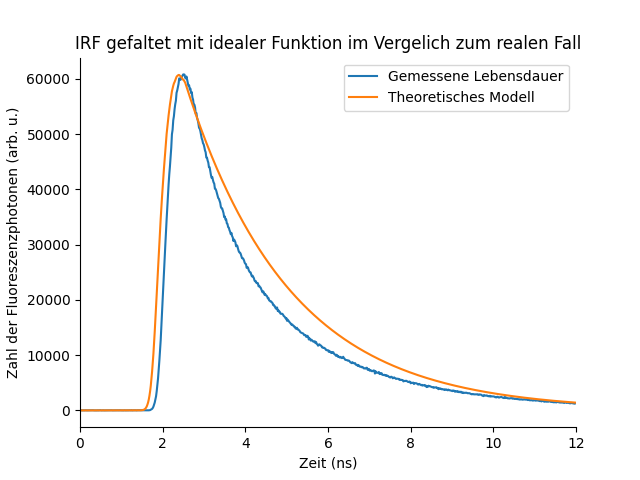
\includegraphics[width = \linewidth]{Bilder/Auswertung/IRFProgConvol.png}
    \caption{Lebensdauer bei Einzelphotonenereignissen und die Faltung der IRF (Programmgeneriert) und dem idealen Signal ($\tau_{YFP}$ unkorrigiert) nach der Totzeit. }
    \label{bild:IRFconvProg}
\end{figure}


\begin{figure}[h]
    \centering
    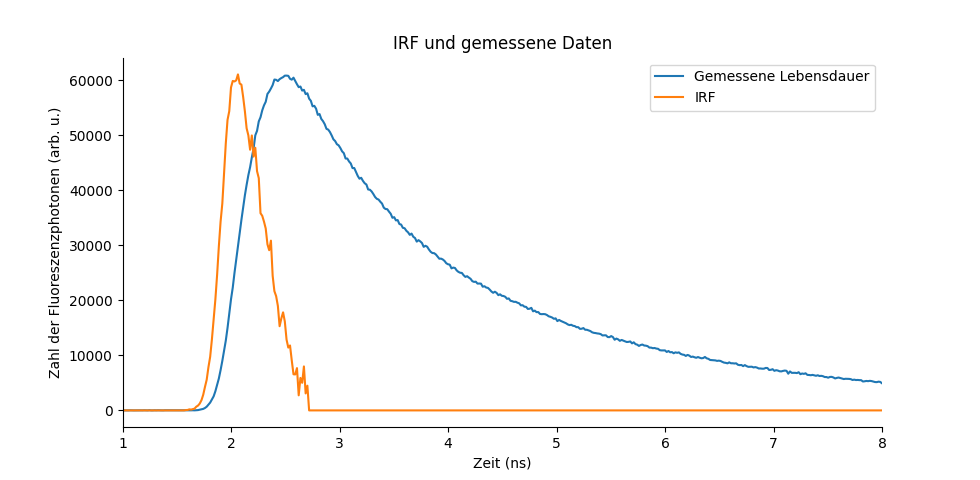
\includegraphics[width = \linewidth]{Bilder/Auswertung/IRFProg.png}
    \caption{ Lebensdauer bei Einzelphotonenereignissen und IRF durch das Programm 'SymPhoTime' generiert. Man sieht eine unsymmetrische Form.}
    \label{bild:IRFProg}
\end{figure}



\clearpage
\section{Protokoll}
\label{section:Protokoll}
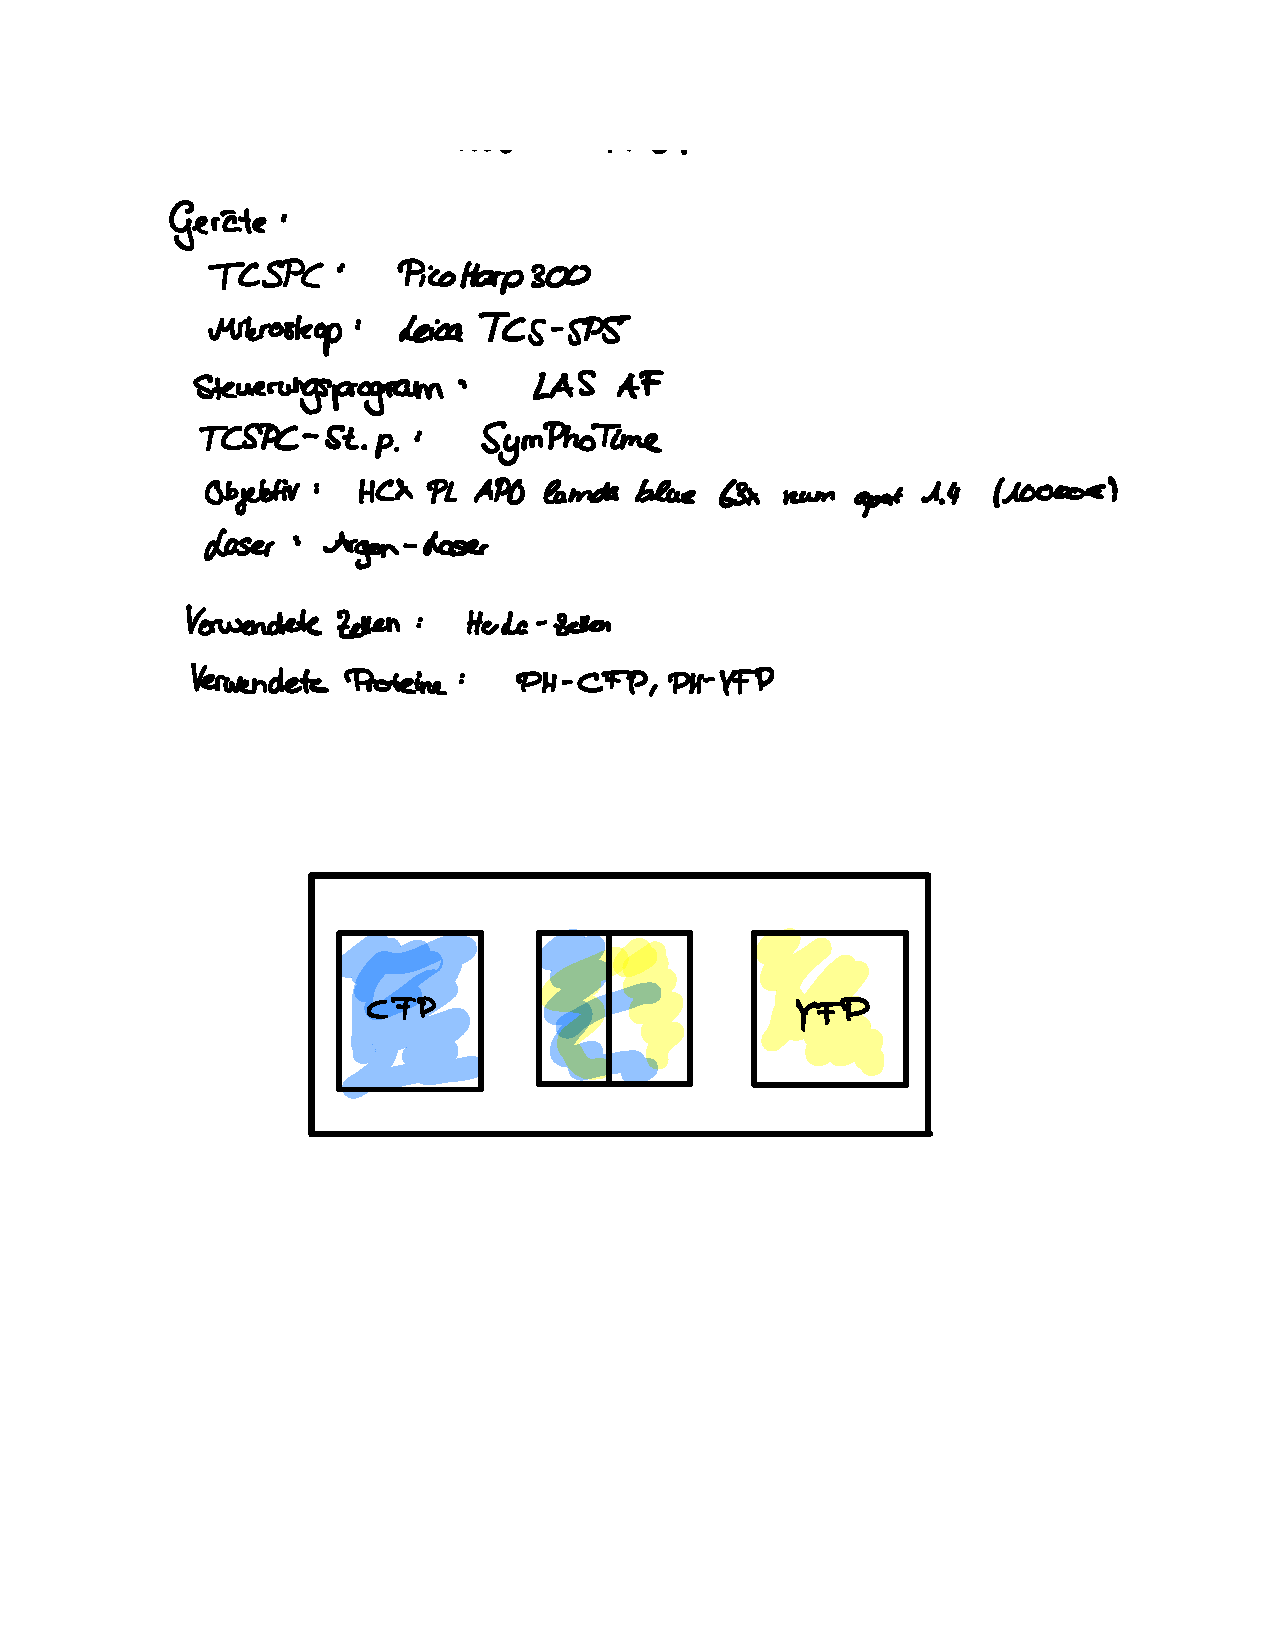
\includepdf[pages = 1-6]{FRETProt.pdf}
